\section{Results} \label{section:results}
In the following sections, results from running the AMPL implementation and both heuristics will be presented. The parameter values used in the runs will also be given. 

\subsection{AMPL implementation}\label{sec:ampl_res}

By implementing the given mathematical model in AMPL and solving it with CPLEX 12.5, provides the values displayed in Table \ref{tab:CPLEX_res}. The weights in Equation \ref{objfcn} and \ref{constr:s_min} were set to $L = 2$, $A = 1$, $M =100$ and $N=1$, thus making librarians twice as valuable as assistants and stand-ins 100 times more valuable than no shift changes. 

\begin{table}[!h]
\centering
\caption{Results from solving the mathematical model with CPLEX solver.}
\label{tab:CPLEX_res}
\begin{tabular}{|l|p{3cm}|p{3cm}|l|}
\hline
\rowcolor{Gray} & \textbf{Min num stand-ins (lib, ass)} & \textbf{Stand-in cost} & \textbf{Solution time} \\ \hline
\cellcolor{Gray} \textbf{Result} & \multicolumn{1}{c|}{(3,0)} & \multicolumn{1}{c|}{6} & \multicolumn{1}{c|}{19 min} \\
\hline
\end{tabular}
\end{table}

Only the stand-in part of the objective function is presented, since this value can be used as a benchmark in measuring the performance of the heuristics. The number of shift changes, which is the second part of the objective function in Equation \ref{objfcn}, is zero.

\subsection{Week block scheduling approach}
As most of the costs are correlated with each other, some parameter tuning was required. The final result of the parameter tuning are shown in Table \ref{tab:cost_parameters}. Their respective descriptions can be seen in Table \ref{tab:all_costs}. 

\begin{table}[!h]
\centering
\caption{List of all costs used in the week block scheduling approach and their respective values.}
\label{tab:cost_parameters}
\begin{tabular}{|c|c|}
\hline
\rowcolor[HTML]{FD6864} 
\multicolumn{2}{|l|}{\cellcolor{corn} \textbf{Demand costs}} \\ \hline
%\multicolumn{2}{|c|}{\cellcolor[HTML]{FD6864}Demand costs}    \\ \hline
\rowcolor[HTML]{C0C0C0} 
Cost name                                      & Cost value       \\ \hline
Demand\_few\_ass                        & 350         \\ \hline
Demand\_few\_lib                        & 300         \\ \hline
Demand\_many\_ass                       & 200         \\ \hline
Demand\_many\_lib                       & 40          \\ \hline
Demand\_few\_total                             & 800         \\ \hline
Demand\_many\_total                            & 700         \\ \hline
Demand\_evening\_cost         & 20,000 				\\ \hline
Demand\_PL\_good\_ass        & 1,200            \\ \hline
Demand\_PL\_good\_lib        & 800           \\ \hline
Demand\_PL\_bad\_ass         & 1,200           \\ \hline
Demand\_PL\_bad\_lib         & 1,600             \\ \hline
\rowcolor[HTML]{FD6864} 
\multicolumn{2}{|l|}{\cellcolor{corn} \textbf{PL costs}} \\ \hline
\rowcolor[HTML]{C0C0C0} 
Cost name                                      & Cost value       \\ \hline
PL\_good\_amount                  & 1,000                   \\ \hline
PL\_violate\_amount             & 1,500                  \\ \hline
\rowcolor[HTML]{FD6864} 
\multicolumn{2}{|l|}{\cellcolor{corn} \textbf{Weekend costs}} \\ \hline
\rowcolor[HTML]{C0C0C0} 
Cost name                                      & Cost value       \\ \hline
HB\_amount                       & 15,000    \\ \hline
No\_weekend                & 5,000                   \\ \hline
\rowcolor[HTML]{FD6864} 
\multicolumn{2}{|l|}{\cellcolor{corn} \textbf{Stand-in costs}} \\ \hline
\rowcolor[HTML]{C0C0C0} 
Cost name                                      & Cost value       \\ \hline
Stand\_in\_cost                     & 5     \\ \hline
\end{tabular}
\end{table}

Worth noting is that these values are most certainly not the best possible, as they have mostly been assigned using intuition. However, a few relations were determined by either running tests or using reasoning. An example is if $PL\_good\_cost > Demand\_PL\_good\_ass$ or $PL\_good\_cost > Demand\_PL\_good\_lib$. If one of those holds, all staff members that is able to be assigned another PL, without violating the individual PL assigment constraint, will be. Thereby, leaving the library overstaffed with staff members assigned to PL. The reason is because the net of $-PL\_good\_cost + Demand\_PL\_good\_ass/lib$ will be negative, meaning it is preferable to assign yet another PL to a staff member, regardless of how many there already are assigned. This leads to an overstaffed library on some days, and lack of staff members on other days.

Table \ref{successful_iter} shows the success rate of finding a solution during a script execution. A run is considered to fail, if no feasible solution is found during the final phase. This script execution is using the cost parameters shown in Table \ref{tab:cost_parameters}. 
\begin{table}[!h]
\centering
\caption{Number of successful runs. A failed run is when no feasible solution is found during the final phase.}
\label{successful_iter}
\begin{tabular}{|c|c|}
\hline
Successful runs         & 420      \\ \hline
Runs (total) & 638      \\ \hline
\%                 & $\sim$66 \\ \hline
\end{tabular}
\end{table}

Table \ref{tab:stand_in_spread} shows statistics of how many stand-ins were found after 420 successful runs. In case "No stand-ins" are found after a run, then a feasible solution is found, however, there are no stand-ins on the worst day (or days). The results "1 assistant" or "1 librarian" mean that one stand-in was found at best on the worst day (or days).
\begin{table}[!h]
\centering
\caption{Number of stand-ins found in 420 successful runs.}
\label{tab:stand_in_spread}
\begin{tabular}{|c|c|}
\hline
\rowcolor[HTML]{D2D2D2} 
Stand-in spread & Times \\ \hline
No stand-ins    & 351                      \\ \hline
1 assistant     & 33                      \\ \hline
1 librarian 	& 36 \\ \hline
\end{tabular}
\end{table}

Figure \ref{fig:feasibleRerun} shows a plot of the objective function value after destroy and repair iterations. When the value on the y-axis reaches zero, a feasible solution is found. Whenever an iteration is below the final phase boundary, the entering criterion is checked. If the final phase is entered, the few existing demand violations will be taken care of, one by one, by assigning the stand-ins where the violations occur. The final phase boundary is set as $1\cdot10^4$.

Every time the value skyrockets, a solution has been discarded in the final phase. Empty blocks are, thereafter, assigned to all staff members and the run is once again entering the destroy and repair loop. Destroy and repair iterations are being executed until a solution is likely to be found, that is, there are enough stand-ins available to take care of the demand violations. 

%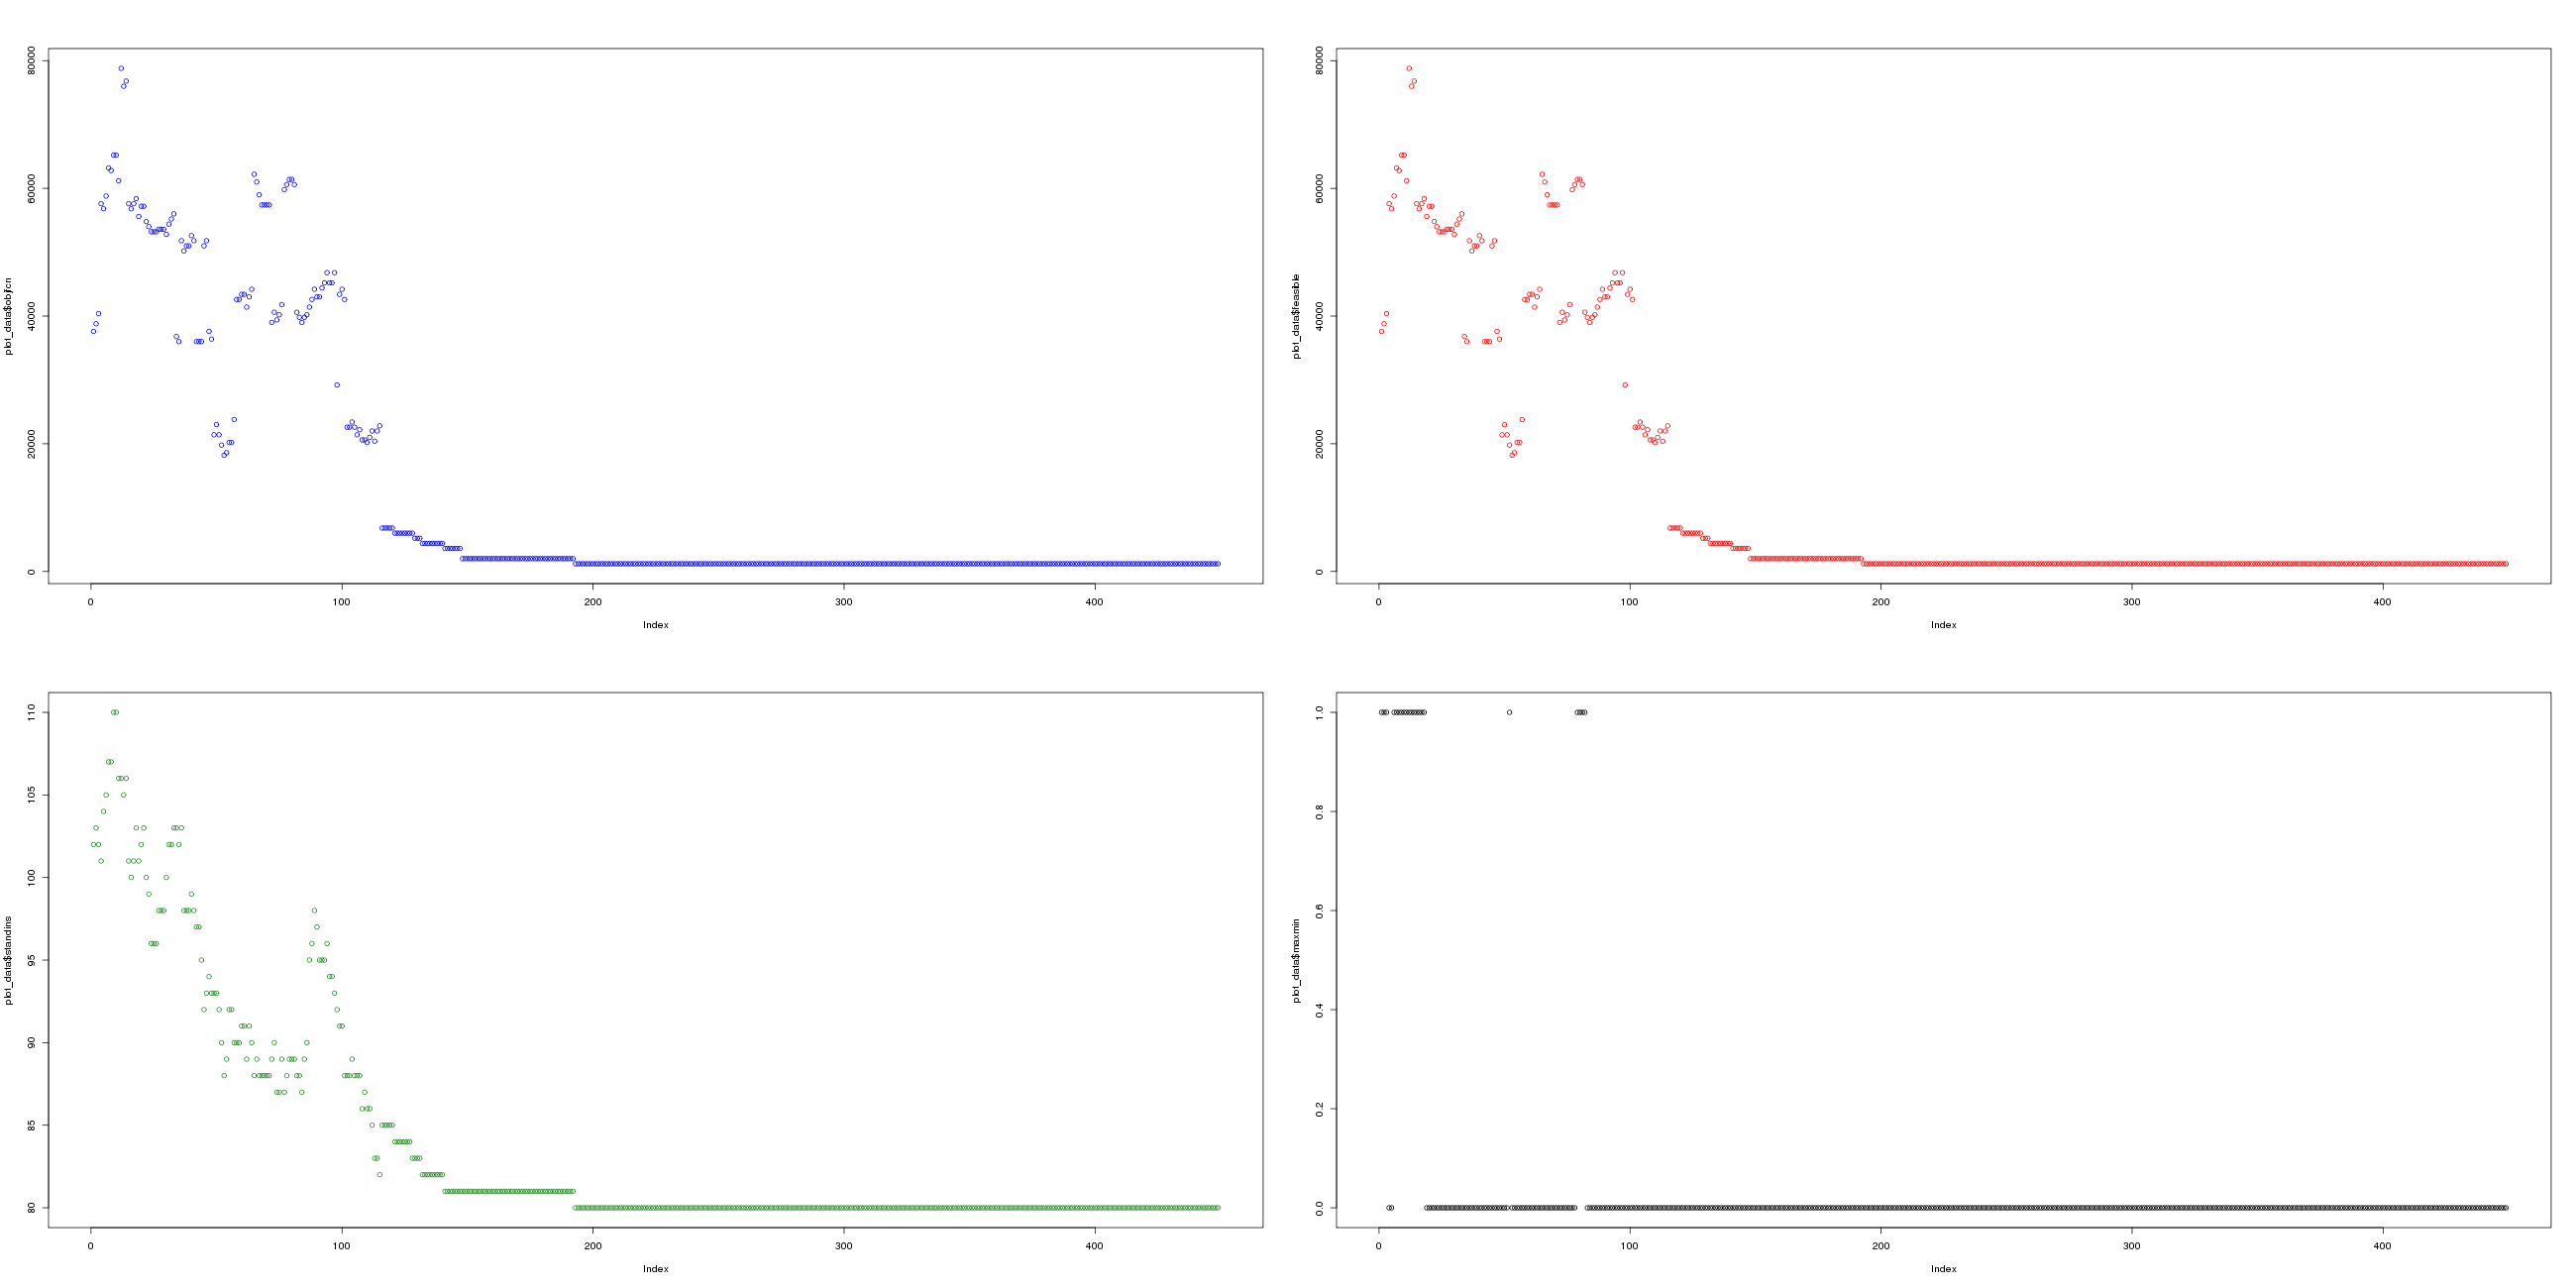
\includegraphics[scale = 0.3, width = 15cm]{Rplot}
%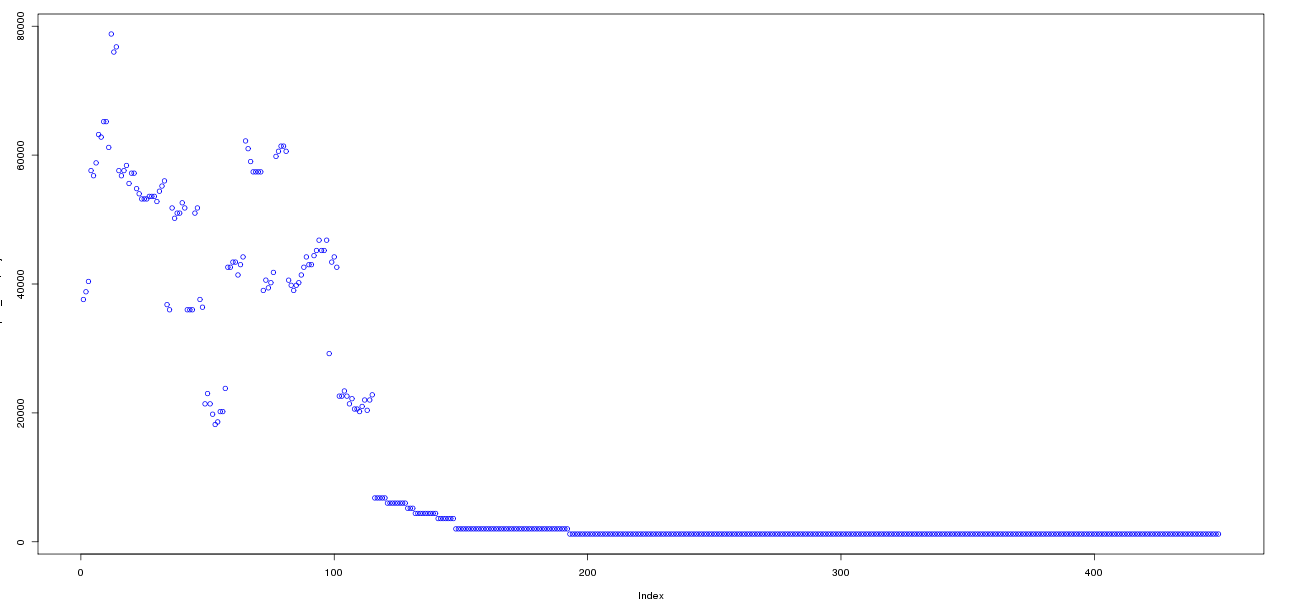
\includegraphics[scale = 0.3, width = 15cm]{1Plot}
\begin{figure}[!h]
\centering
%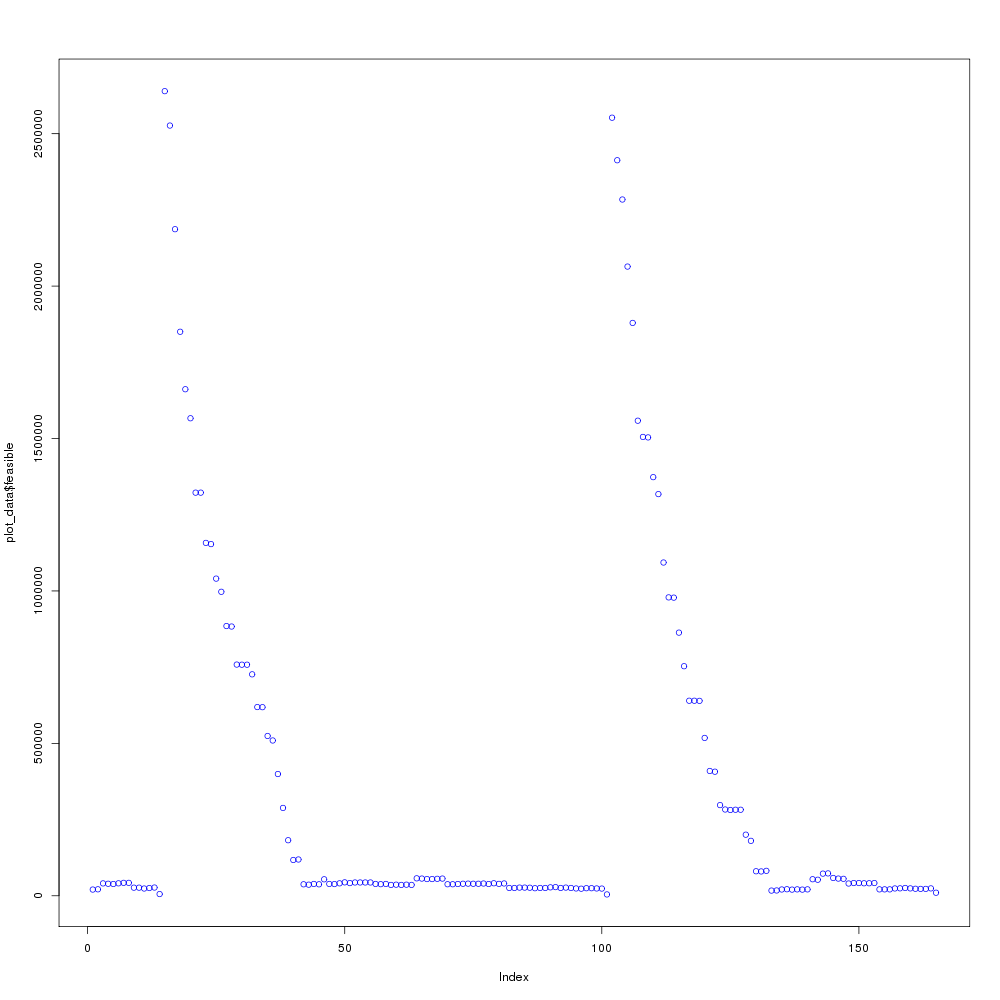
\includegraphics[scale = 0.3]{Chapters/ImagesClaes/Rfeasible.png}
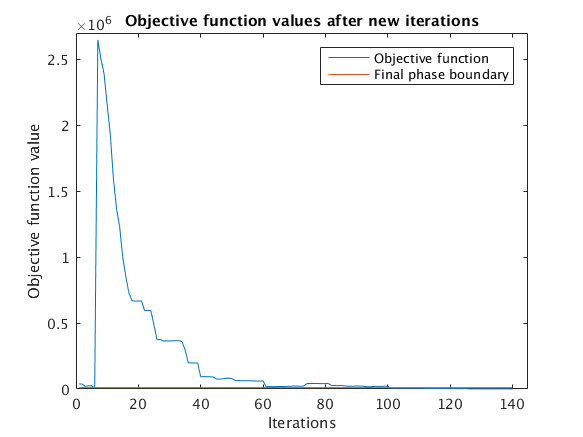
\includegraphics[scale = 0.8]{Chapters/ImagesClaes/1phase1iter1ReRun.png}
\caption{Plot of the objective function value after destroy and repair iterations; one time without enough stand-ins, when trying to enter the final phase.}
\label{fig:feasibleRerun}
\end{figure}

As seen in Figure \ref{fig:feasibleRerun} there are not enough stand-ins one time during the run. What happens is that the objective function gets below the final phase boundary, but does not meet the stand-in criterion and, therefore, destroys every workers' schedule. 

Figure \ref{fig:feasibleNoRerun} illustrates a run when there are enough stand-ins to enter the final phase.

\begin{figure}[!h]
	\centering
	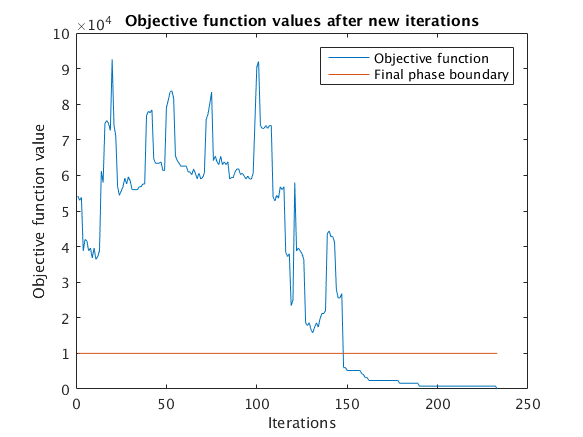
\includegraphics[scale = 0.8]{Chapters/ImagesClaes/1phase1iterNoReRun.png}
	\caption{Plot of the objective function value after destroy and repair iterations with enough stand-ins when trying to enter the final phase.}
	\label{fig:feasibleNoRerun}
\end{figure}

To illustrate why the solution gets worse after a destroy and repair iteration; consider the case when two librarians with the same rotation are being repaired, where one only can work at HB during weekends and the other one can work at either HB or with Desk tasks. If the more versatile librarian is repaired first and being assigned to HB, due to the cost parameters, then it will be impossible for the second librarian to be assigned any weekend tasks. This results in a high cost contribution to the objective function value.

\subsection{Task allocation approach}\label{sec:task_dist_res}

In order to find a good value for the weights described in Section \ref{subsection:tasks_cost}, different tuning tests were performed. These tests resulted in the weights presented in Table \ref{tab:tasks_weight}. These weights are used in all test in this section unless stated otherwise.

\begin{table}[!h]
\centering
\caption{Weights used in the implementation.}
\label{tab:tasks_weight}
\begin{tabular}{|l|l|}
\hline
\rowcolor{gray!90} \textbf{Weight} & \textbf{Weight value} \\ \hline
\multicolumn{2}{|l|}{\cellcolor{Gray} \textbf{Weekend Objective Function Weights}} \\ \hline
$W_{SI\_m}$ & 0.1 \\ \hline
$W_{S\_m}$ & 0.1 \\ \hline
$W_{D\_m}$ & 10 \\ \hline
$W_{SI\_a}$ & 0.01 \\ \hline
$W_{S\_a}$ & 0.01 \\ \hline
$W_{D\_a}$ & 1 \\ \hline
\multicolumn{2}{|l|}{\cellcolor{Gray} \textbf{Staff Member/Staff Member Objective Function Weights}} \\ \hline
$W_{w\_SI}$ & 
\begin{tabular} [x]{@{}c@{}}
	2 \text{if librarian} \\ 
	1 \text{if assistant}
\end{tabular} \\ \hline
$W_{Task\_D}$ / $W_{w\_Task\_D}$ & 100\\ \hline
$W_{Task\_W}$ / $W_{w\_Task\_W}$ & 	10 \\ \hline
$W_{PL\_W}$ / $W_{w\_PL\_W}$ & 5 \\ \hline
$W_{PL\_Tot}$ / $W_{w\_PL\_Tot}$ & 5 \\ \hline
$W_{SShift\_W}$ / $W_{w\_SShift\_W}$ & 4 \\ \hline
\end{tabular}
\end{table}



The first six weights, belonging to the weekend objective function, were most experimented with and will be discussed further in this section. The first three, the min weights, are scaled relatively to each other and decide how much weight is placed on maximizing the number of stand-ins during the worst day, maximizing the number of staff members at the worst day and maximizing the number of staff members at the worst shift, respectively. Only maximizing the number of stand-ins at the worst day during the weekend phase would not give a complete estimation of the number of stand-ins in the final schedule, since this number also depends on how many workers are present in total during that day and during the shifts of the days. Thus, all three aspects were measured.

The next three weights, refered to as the average weights, belong to the three costs which give the average of each of the three aspects described above. They are simply calculated as one tenth of their equivalent min weights. The weights in Equation \ref{eq:wend_cost_calc}, $W_{lib}$ and $W_{ass}$ were set to $2$ and $1$, respectively, since it can be argued that one librarian can perform twice as many tasks as one assistant.

The individual staff member cost and the staff member objective function costs, which measure the same aspects of the schedule, have been given the same weights, as is illustrated in Table \ref{tab:tasks_weight}. This is due to the fact that these weights, relative to each other, decide what constraints are most strict. It is, for example more severe to break the rule of one task per day, than to break the rule of having too many shifts at the same time in a week, which is reflected in the weights. The stand-in weight $W_{w\_SI}$ is twice as high for librarians as for assistant.

The two phases of the implementation are run a specified number of iterations, referred to as $It_{wend}$ and $It_{wday}$. These parameters were also trimmed and the results from different iteration values are displayed in Tables \ref{tab:taskdist_res_wendit} and \ref{tab:taskdist_res_wdayit}. The results for weight tuning are displayed in Table \ref{tab:taskdist_weights_res}.

\begin{table}[!h]
\centering
\caption{Results from the task allocation heuristic when varying $It_{wend}$}
\label{tab:taskdist_res_wendit}
\begin{tabular}{|l|l|l|}
\hline
\rowcolor{Gray} \textbf{$It_{wend}/It_{wday}$} &  \textbf{Heuristic cost} &  \textbf{AMPL cost} \\ \hline
\cellcolor{Gray} \textbf{10/10} & \multicolumn{1}{c|}{4.40} & \multicolumn{1}{c|}{4.78} \\
\cellcolor{Gray} \textbf{50/10} & \multicolumn{1}{c|}{5.00} & \multicolumn{1}{c|}{5.34} \\
\cellcolor{Gray} \textbf{100/10} & \multicolumn{1}{c|}{5.26} & \multicolumn{1}{c|}{5.52} \\
\cellcolor{Gray} \textbf{500/10} & \multicolumn{1}{c|}{5.66} & \multicolumn{1}{c|}{5.78} \\
\cellcolor{Gray} \textbf{1000/10} & \multicolumn{1}{c|}{5.54} & \multicolumn{1}{c|}{5.66}  \\
\hline
\end{tabular}
\end{table}

\begin{table}[!h]
\centering
\caption{Results from the task allocation heuristic when varying $It_{wday}$}
\label{tab:taskdist_res_wdayit}
\begin{tabular}{|l|l|l|}
\hline
\rowcolor{Gray} \textbf{$It_{wend}/It_{wday}$} &  \textbf{Heuristic cost} &  \textbf{AMPL cost} \\ \hline
\cellcolor{Gray} \textbf{500/5} & \multicolumn{1}{c|}{5.47} & \multicolumn{1}{c|}{5.74} \\
\cellcolor{Gray} \textbf{500/10} & \multicolumn{1}{c|}{5.66} & \multicolumn{1}{c|}{5.78} \\
\cellcolor{Gray} \textbf{500/15} & \multicolumn{1}{c|}{5.6} & \multicolumn{1}{c|}{5.74} \\
\cellcolor{Gray} \textbf{500/20} & \multicolumn{1}{c|}{5.57} & \multicolumn{1}{c|}{5.74} \\
\hline
\end{tabular}
\end{table}


\begin{table}[!h]
\centering
\caption{Results from the task allocation heuristic when varying weights. Here, $It_{wend} = 1000$ and $It_{wday} = 20$ in all runs.}
\label{tab:taskdist_weights_res}
\begin{tabular}{|l|l|l|}
\hline
\rowcolor{Gray} \textbf{$W_{SI\_m}/W_{S\_m}/W_{D\_m}$} & \textbf{Heuristic cost} &  \textbf{AMPL cost} \\ \hline
\cellcolor{Gray} \textbf{0/0/0 }& \multicolumn{1}{c|}{2.85} & \multicolumn{1}{c|}{3.66}  \\
\cellcolor{Gray} \textbf{1/1/1} & \multicolumn{1}{c|}{5.43} & \multicolumn{1}{c|}{5.54}  \\
\cellcolor{Gray} \textbf{10/0.1/0.1} & \multicolumn{1}{c|}{5.11} & \multicolumn{1}{c|}{5.36}  \\
\cellcolor{Gray} \textbf{0.1/10/0.1} & \multicolumn{1}{c|}{5.43} & \multicolumn{1}{c|}{5.60}  \\
\cellcolor{Gray} \textbf{0.1/0.1/10} & \multicolumn{1}{c|}{5.57} & \multicolumn{1}{c|}{5.80} \\
\hline
\end{tabular}
\end{table}

The tables display two costs for each test, the heuristic cost and the AMPL cost. These are calculated as the average result of 100 runs. Each run takes between a few seconds and a few minutes to perform. The heuristic cost is the actual result of the heuristic, measuring how well the heuristic solves the problem. The AMPL cost is the result obtained when solving the problem to optimality in CPLEX, using the weekend work pattern found in the heuristic. Thus, this value measures how good the weekend phase works. Both figures should be compared to the optimal stand-in value for the problem, which is 6 (see Table \ref{tab:CPLEX_res}).

Studying Table \ref{tab:taskdist_res_wendit}, it can be seen that the AMPL cost increases with more weekend iterations. However, after 500 iterations, the cost stops to improve and it is actually deteriorating slightly. This is probably indicating that the weekend objective function value can only give a rough measure of a good schedule, and the result does not only depend on the number of iterations but also on chance. 

Similarly, in Table \ref{tab:taskdist_res_wdayit}, the heuristic cost increases until a certain threshold, when the solutions are not improving any more. This might indicate that the second phase is not random enough, so the same schedules are found multiple times. This might be solved through implementing varying weights or introducing more randomness in task placement.

Table \ref{tab:taskdist_weights_res} shows the results from using a few extreme weight combinations. It is is clear from the table that, although the performance does not vary to any larger extent when shifting the focus in the weights, using a completely random search with no weights produces poor results. The last combination of weights seems to be performing slightly better than the others, and thus these weights were chosen in the implementation.

The weekend objective function value during a typical run is shown in Figure \ref{fig:obj_fun_vals}. The effects of the SA accept function are visible in the plot as smaller or larger dives in the objective function value. In the runs, the SA parameters $T_0 = 0.4$ and $\alpha = 0.985$. $It_{wend} = 1000$ were used. The graph suggests that a high weekend objective function value is found already within the 200 first iterations, which is consistent with the results in Table \ref{tab:taskdist_res_wendit}.

\begin{figure}[!htbp]
\centering
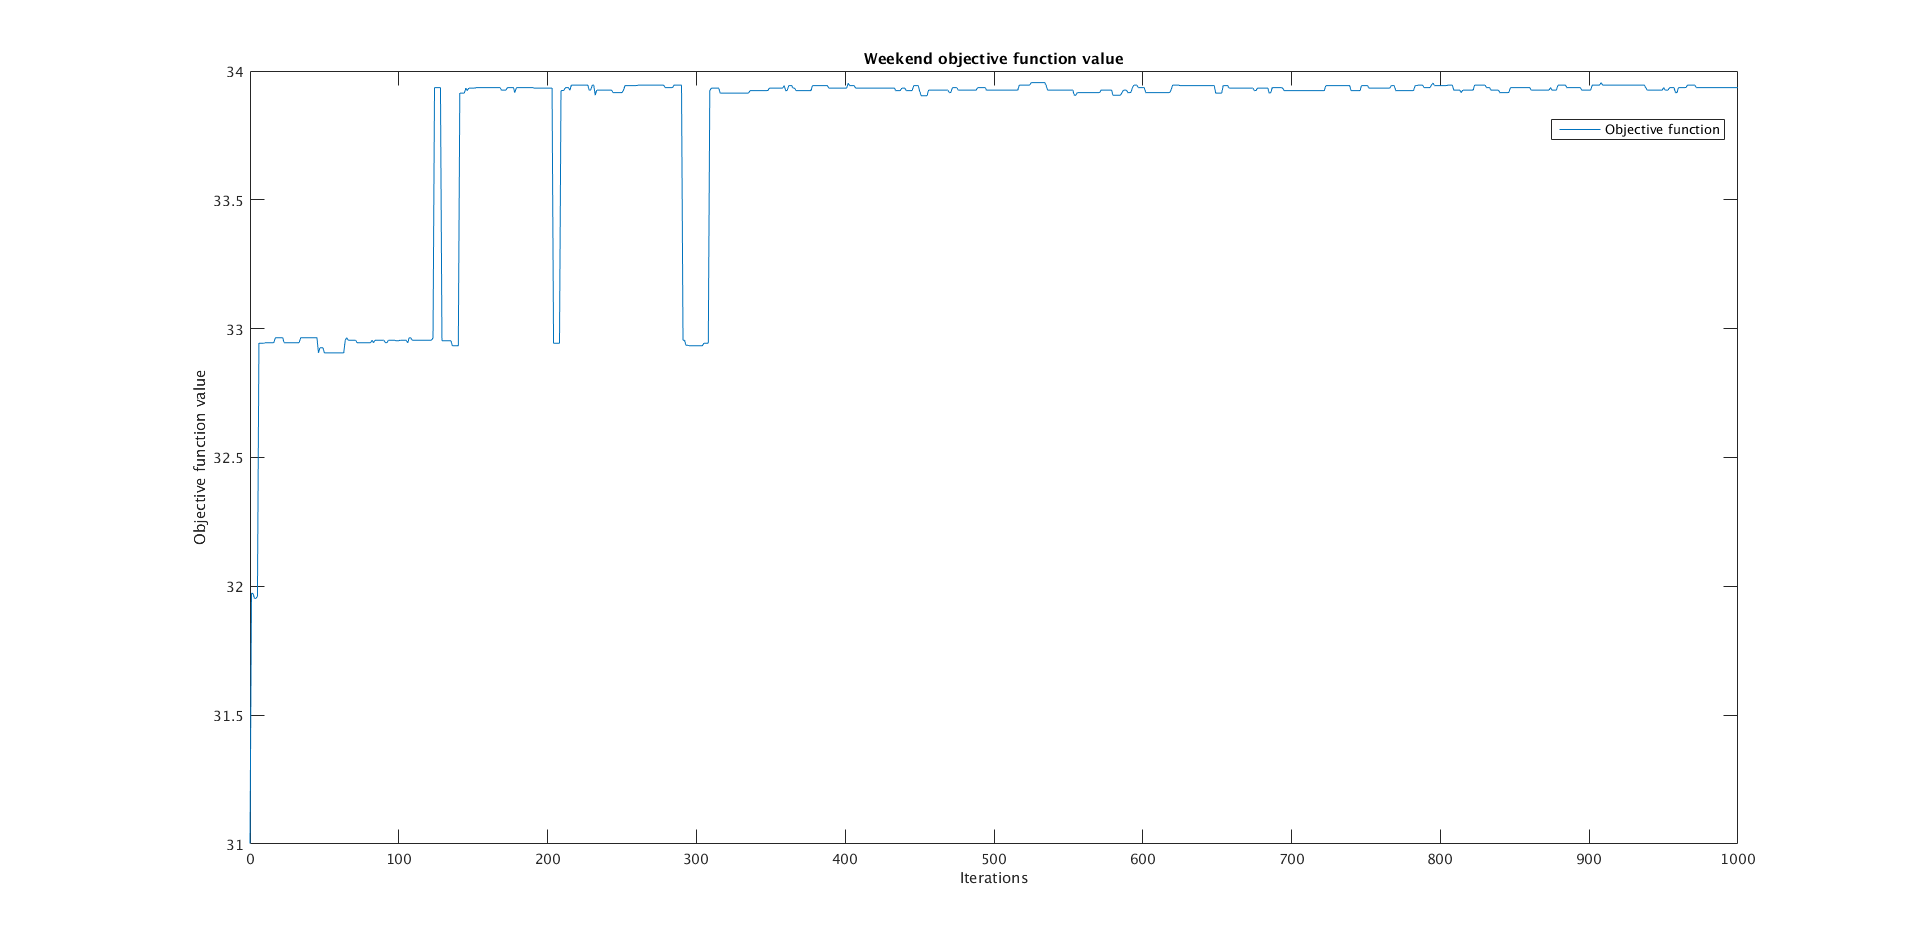
\includegraphics[width=0.9\textwidth, trim = 100px 0px 100px 20px, clip]{Chapters/ImagesEmelie/Plot_1000_20.png}
\caption{The weekend objective function for 1000 iterations}
\label{fig:obj_fun_vals}
\end{figure}


\begin{figure}[!htbp]
\centering
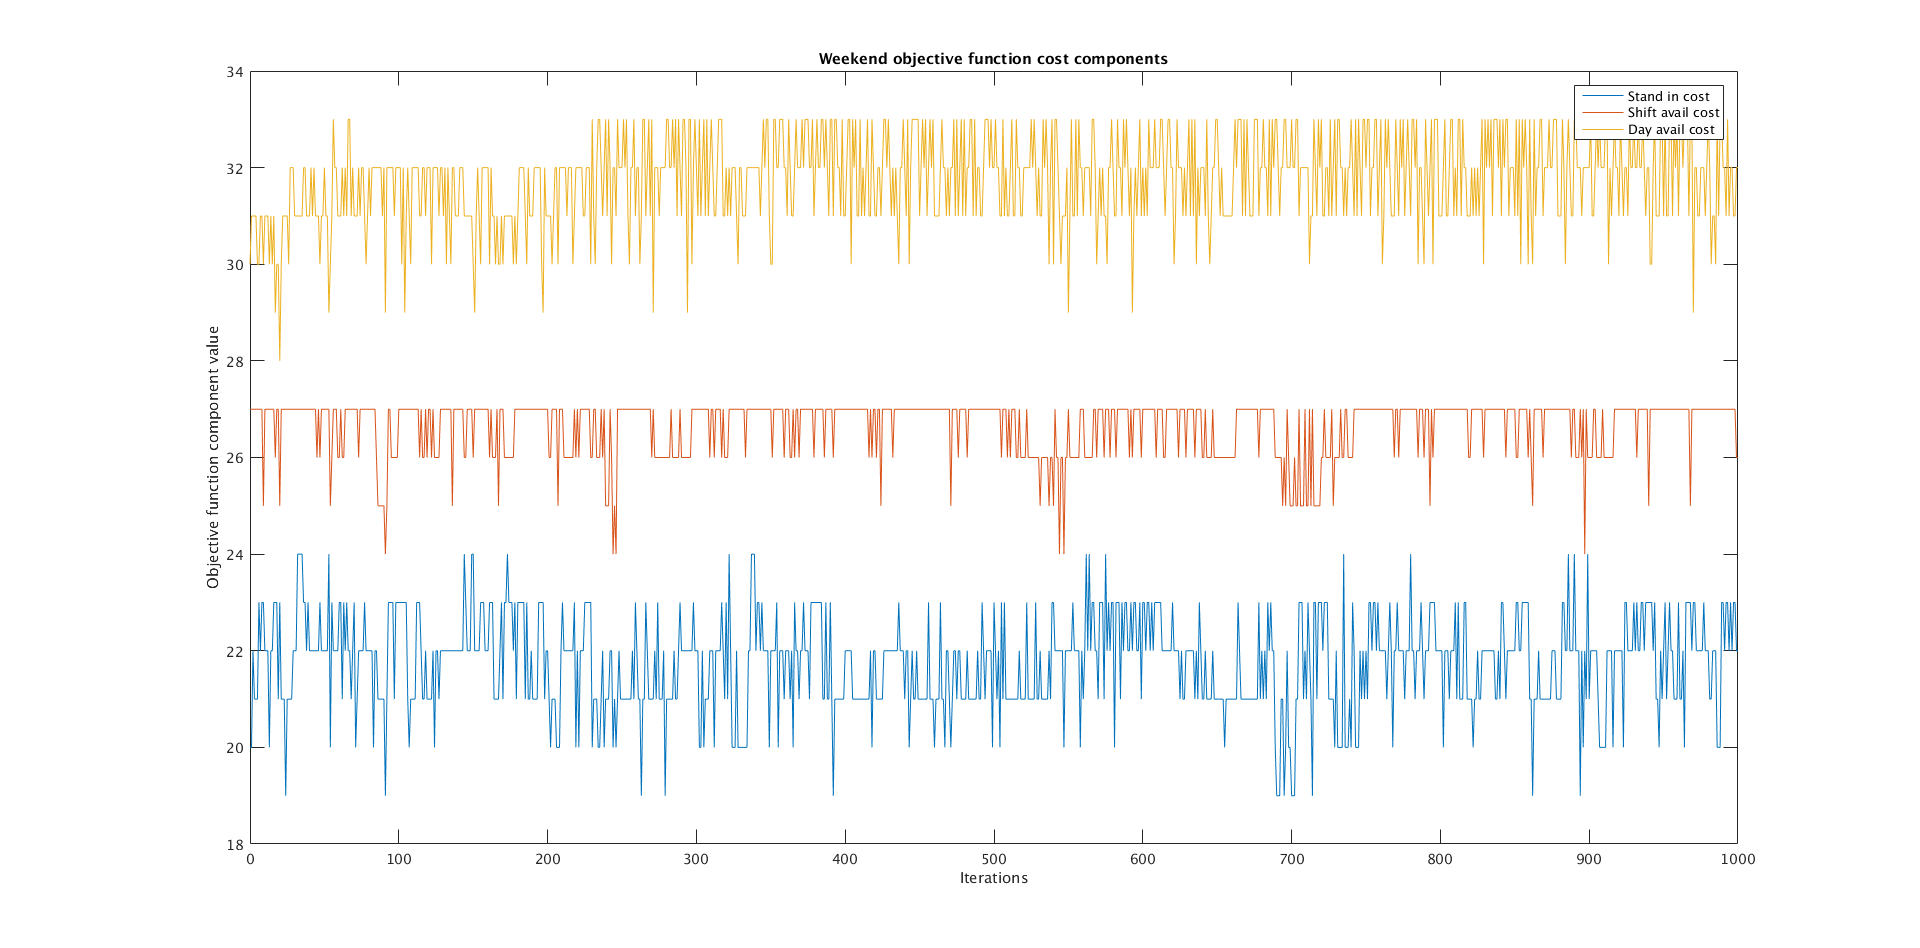
\includegraphics[width=0.9\textwidth, trim = 100px 0px 100px 20px, clip]{Chapters/ImagesEmelie/Components_1000_20.png}
\caption{The weekend objective function minimum cost components for 1000 iterations}
\label{fig:obj_fun_comp}
\end{figure}

\begin{figure}[!h]
\centering
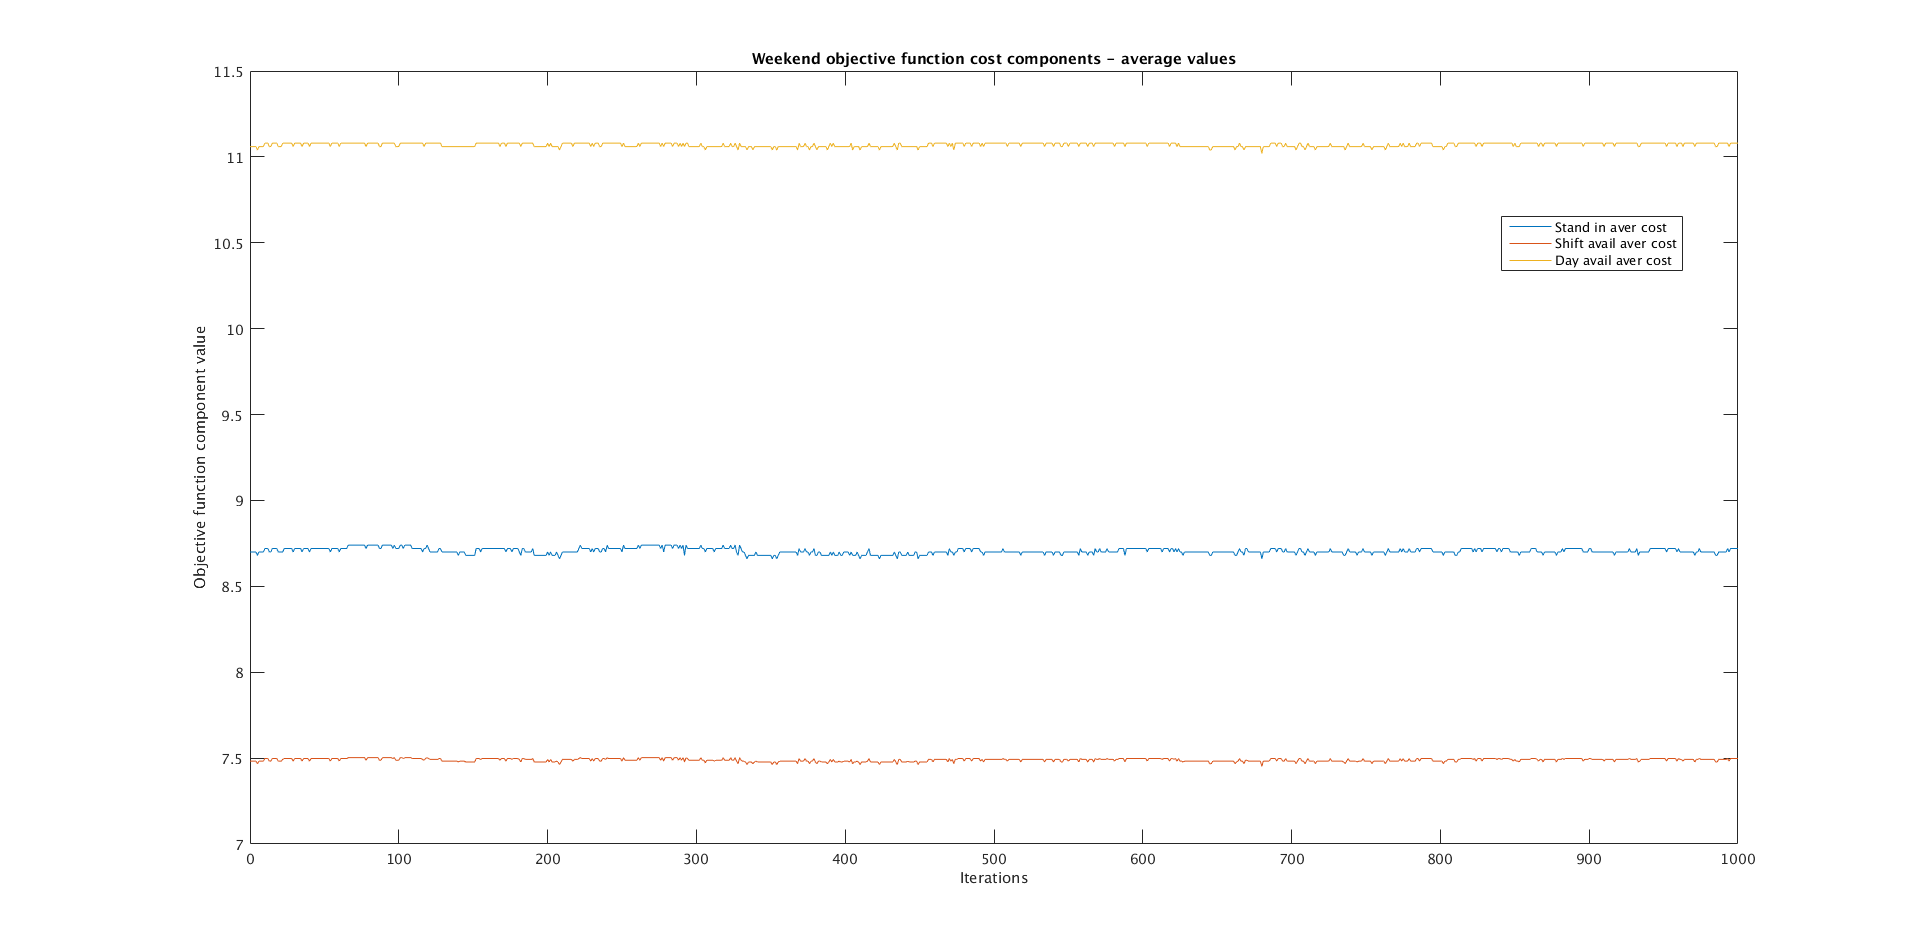
\includegraphics[width=0.9\textwidth, trim = 100px 0px 100px 20px, clip]{Chapters/ImagesEmelie/Components_av_1000_20.png}
\caption{The weekend objective function average costs components for 1000 iterations}
\label{fig:obj_fun_comp_aver}
\end{figure}


In Figure \ref{fig:obj_fun_comp} and Figure \ref{fig:obj_fun_comp_aver}, the three different cost components of the weekend objective function for the same run are displayed. In the first plot, the minimum costs are displayed. These seem to move between a few discrete values, although a small improvement over the iterations can be seen, at least in the day avail cost component. The average values are almost constant throughout the iterations, as can be seen in the second plot. This is probably due to the fact that the total number of available staff members barely changes when shifting their weeks.

Attempts were made to correlate the min component values of the weekend objective function to each other. However, the results were fluctuating between different runs so no clear correlations could be identified. This suggests that they are measuring three independent aspects.

\section{Discussion}
In this section, the heuristic results, presented in Section \ref{section:results}, will be discussed. Pros and cons for both methods are given, so that they can be more easily compared.


\subsection{Week block scheduling approach}
Table \ref{tab:pros_cons_weekly_scheduling} lists pros and cons with the implemented week block scheduling approach. Some pros and cons were considered before this heuristic was chosen. Mainly, the con concerning the exponential growth of week blocks was taken into consideration, and an estimate of the upper limit of the problem size was done.

The pro regarding the same amount of week blocks was taken into consideration, as the heuristic was thought of having firstly, a block construction phase and secondly, an assignment phase. However, the most significant pro of this approach is that many of the constraints are already met, implicitly, when the blocks are created. Constraints like maximum of one task per day, one evening per week, one PL per week, two shifts at the same hour per week and more are already taken care of. 

Cons like rotations, solution time and costs are no major issues, as they can be avoided by a few smarter implementations. For instance, rotations can be improved by assigning a chosen value whenever a staff member is available as stand-in on a day. From the sum of those values an even distribution of possible stand-ins can be acquired by, for instance, always letting the difference between the lowest and the highest sum of stand-ins, through the days, be as small as possible. This improvement should be done instead of randomly generating the new rotations in the destroy and repair iteration. 

The improvement mentioned above should also implicitly decrease the solution time, as less iterations would be required to find a feasible solution.

In contrast to the cons mentioned above, a major issue is to always be able to create a pool of possible week block appearances, regardless of the problem size. Just by adding meetings and the assignment of the library on wheels tasks would make the number of possible week block appearances grow considerably.

\begin{table}[H]
\caption{Pros and cons with the implemented week block scheduling approach.}
\label{tab:pros_cons_weekly_scheduling}
\begin{tabularx}{\linewidth}{>{\parskip1ex}X@{\kern4\tabcolsep}>{\parskip1ex}X}
\toprule
\hfil\bfseries Pros
&
\hfil\bfseries Cons
\\\cmidrule(r{3\tabcolsep}){1-1}\cmidrule(l{-\tabcolsep}){2-2}

%% PROS, seperated by empty line or \par
Many constraints are already met, implicitly, when the blocks are created. \par
The same number of week block appearances will exist for five and ten weeks.\par
Quick iterations when destroying and repairing.\par

&

%% CONS, seperated by empty line or \par
Rotations need to be assigned in a systematic way in order to achieve reasonable results, regarding lowest number of stand-ins through the days.\par
The number of unique week block appearances grows exponentially in case more task types are added, such as meetings.\par
The solution time can vary considerably, as several random number generators have been used.\par
More cost parameters are needed for this heuristic, where every one of them affect the solution procedure.

\\\bottomrule
\end{tabularx}
\end{table}

 

\subsection{Task allocation approach}
The results from the previous section point to the fact that finding a good weekend allocation is essential in order to get a good final schedule. When $It_{wend}$ is increased the results improve, up to a limit of around 500 iterations. The results are comparable to those of the AMPL implementation. This suggests that the weekend objective function used gives a weekend schedule which, with a high probability, can provide a good basis for creating the complete schedule. However, it only gives an indication, not an optimal solution, as the results seem to converge to a value slightly lower than the AMPL result. 

Table \ref{tab:taskdist_weights_res} suggests that the weights used in the weekend objective function are important for how well the implementation works, but only to a certain degree. More testing could be done on the weights in order to see if the result can be further improved. However, since the objective function is an incomplete measure of a good schedule the results will never be completely optimal. This is listed as the main drawback in the cons column in Table \ref{tab:pros_cons_task_scheduling}. 

\begin{table}[!ht]
\caption{Pros and cons with the implemented task allocation approach}
\label{tab:pros_cons_task_scheduling}
\begin{tabularx}{\linewidth}{>{\parskip1ex}X@{\kern4\tabcolsep}>{\parskip1ex}X}
\toprule
\hfil\bfseries Pros
&
\hfil\bfseries Cons
\\\cmidrule(r{3\tabcolsep}){1-1}\cmidrule(l{-\tabcolsep}){2-2}

%% PROS, seperated by empty line or \par
In most cases, the method finds an optimal solution. \par
The method is very fast compared to the CPLEX solver. Only a few iterations in each phase gives good results. \par
The method can be used to find a good weekend schedule. The rest of the schedule can then be created using another method such as CPLEX, in a short time. \par

&

%% CONS, seperated by empty line or \par
The weekend objective function is not an exact measurement of a good weekend schedule. \par
There are many weights and parameters to take into consideration in the implementaion. \par


\\\bottomrule
\end{tabularx}
\end{table}

\iffalse
\begin{table}[!h]
\centering
\label{tab:taskdist_res}
\caption{Results from the task allocation heuristic. Weights from Table \ref{tab:tasks_weight}}
\begin{tabular}{|l|l|l|l|}
\hline
\rowcolor{Gray} \textbf{$It_{wend}/It_{wday}$} &  \textbf{Heuristic cost} &  \textbf{AMPL cost} & \textbf{$\rho_{O\_A}$} \\ \hline
\cellcolor{Gray} \textbf{100/20} & \multicolumn{1}{c|}{5.22} & \multicolumn{1}{c|}{5.48} & 0.58 \\
\cellcolor{Gray} \textbf{500/20} & \multicolumn{1}{c|}{5.64} & \multicolumn{1}{c|}{5.74} & -0.20 \\
\cellcolor{Gray} \textbf{1000/10} & \multicolumn{1}{c|}{5.54} & \multicolumn{1}{c|}{5.66} & 0.03 \\
\cellcolor{Gray} \textbf{1000/20} & \multicolumn{1}{c|}{5.57} & \multicolumn{1}{c|}{5.80} & 0.08 \\
\cellcolor{Gray} \textbf{1000/30} & \multicolumn{1}{c|}{5.50} & \multicolumn{1}{c|}{5.68} & -0.06 \\
\hline
\end{tabular}
\end{table}
\fi
